\documentclass{article}
\usepackage{amsmath}
\usepackage{amssymb}
\usepackage{fancyhdr}
\usepackage[utf8]{inputenc}
\usepackage{tcolorbox}
\usepackage[left=1in, right=1in, top=1.5in, bottom=1in]{geometry}
\usepackage{tikz}
\usepackage{enumerate}
\usepackage{enumitem}
\usepackage{pgfplots}
\usepackage{ragged2e}
\usepackage{tabularx}
\usepackage{array}
\begin{document}
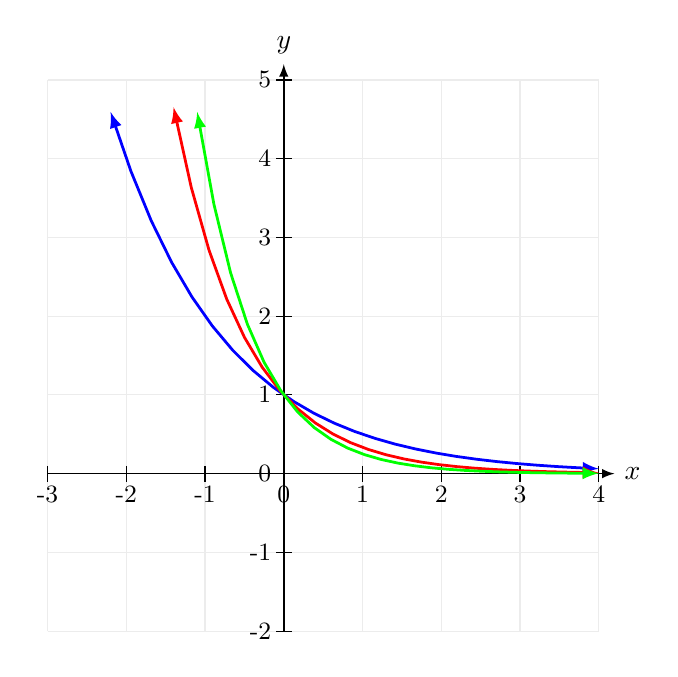
\begin{tikzpicture}[scale=1]
    \draw[gray!15,step=1cm] (-3,-2) grid (4,5);
    \draw[line width=0.2mm, -latex] (-3,0) -- (4.2,0) node[right] {$x$};
    \foreach \x in {-3,...,4} \draw (\x,.1)--(\x,-.1) node[below=1pt, font=\small] at (\x,0) {\x};
    \draw[line width=0.2mm,  -latex] (0,-2) -- (0,5.2) node[above] {$y$};
    \foreach \y in {-2,...,5} \draw (.1,\y)--(-.1,\y) node[left=1pt, font=\small] at (0,\y) {\y};

    % Parabola from (-1,0) to (1,0) with vertex (0,-2)
    \draw[blue, line width=1pt,latex-latex] plot[domain=-2.2:4] (\x,{pow(1/2, \x)});
    \draw[red, line width=1pt,latex-latex] plot[domain=-1.4:4] (\x,{pow(1/3, \x)});
    \draw[green, line width=1pt,latex-latex] plot[domain=-1.1:4] (\x,{pow(1/4, \x)});

\end{tikzpicture}


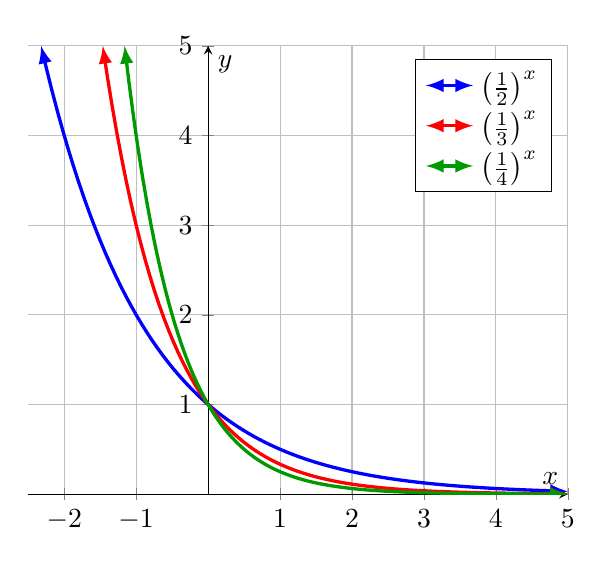
\begin{tikzpicture}
\begin{axis}[
    % Set the exact viewing window for the plot
    xmin=-2.5, xmax=5, % Adjusted xmin to better show the curves from y=5
    ymin=0, ymax=5,     % EXACT y-range from 0 to 5
    % Axis Labels
    xlabel={$x$},
    ylabel={$y$}, % Label for the primary function, or remove
    % Draw axes through the center
    axis lines=middle,
    % Ticks (labeled every 1 unit on x, every 1 unit on y)
    xtick={-2,-1,0,1,2,3,4,5},
    ytick={1,2,3,4,5},
    % Grid lines
    grid=major,
    % Legend
    legend pos=north east, % Or adjust as needed
]

% Blue function: y = (1/2)^x. Starts close to y=5 at x=-1.32.
\addplot[domain={-ln(5)/ln(2)}:5, % Adjusted domain to start near y=5
    samples=100, very thick, blue,latex-latex % Arrowhead at the end of the plot (right side)
] 
{pow(1/2, x)};
\addlegendentry{$\left(\frac{1}{2}\right)^x$}

% Red function: y = (1/3)^x. Starts close to y=5 at x=-0.85.
\addplot[domain={-ln(5)/ln(3)}:5, % Adjusted domain
    samples=100, very thick, red,latex-latex % Arrowhead at the end of the plot
] {pow(1/3, x)};
\addlegendentry{$\left(\frac{1}{3}\right)^x$}

% Green function: y = (1/4)^x. Starts close to y=5 at x=-0.66.
\addplot[domain={-ln(5)/ln(4)}:5, % Adjusted domain
    samples=100, very thick, green!60!black, latex-latex % Arrowhead at the end of the plot
] 
{pow(1/4, x)};
\addlegendentry{$\left(\frac{1}{4}\right)^x$}

\end{axis}
\end{tikzpicture}

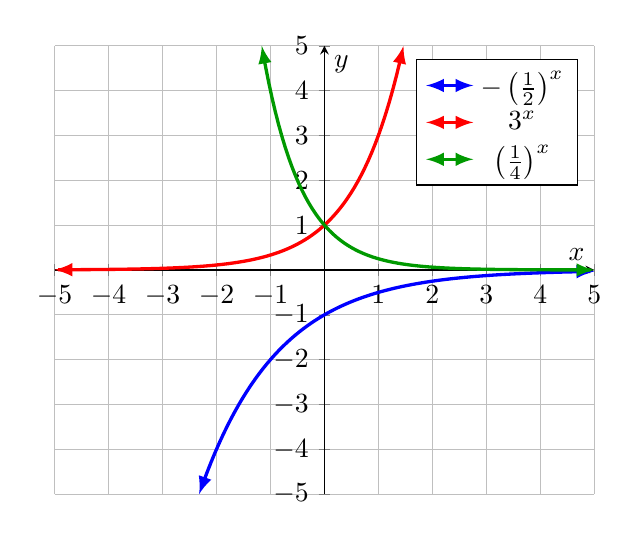
\begin{tikzpicture}
\begin{axis}
[
    % Set the exact viewing window for the plot
    xmin=-5, xmax=5, % Adjusted xmin to better show the curves from y=5
    ymin=-5, ymax=5,     % EXACT y-range from 0 to 5
    % Axis Labels
    xlabel={$x$},
    ylabel={$y$}, % Label for the primary function, or remove
    % Draw axes through the center
    axis lines=middle,
    % Ticks (labeled every 1 unit on x, every 1 unit on y)
    xtick={-5,-4,-3,-2,-1,0,1,2,3,4,5},
    ytick={-5,-4,-3,-2,-1,0,1,2,3,4,5},
    % Grid lines
    grid=major,
    % Legend
    legend pos=north east, % Or adjust as needed
]

% Blue function: y = (1/2)^x. Starts close to y=5 at x=-1.32.
\addplot[domain={-ln(5)/ln(2)}:5, % Adjusted domain to start near y=5
    samples=100, very thick, blue,latex-latex % Arrowhead at the end of the plot (right side)
] 
{-pow(1/2, x)};
\addlegendentry{$-\left(\frac{1}{2}\right)^x$}

% Red function: y = (1/3)^x. Starts close to y=5 at x=-0.85.
\addplot[domain={-5:ln(5)/ln(3)}, % Adjusted domain
    samples=100, very thick, red,latex-latex % Arrowhead at the end of the plot
] {pow(3, x)};
\addlegendentry{$3^x$}

% Green function: y = (1/4)^x. Starts close to y=5 at x=-0.66.
\addplot[domain={-ln(5)/ln(4)}:5, % Adjusted domain
    samples=100, very thick, green!60!black, latex-latex % Arrowhead at the end of the plot
] 
{pow(1/4, x)};
\addlegendentry{$\left(\frac{1}{4}\right)^x$}

\end{axis}
\end{tikzpicture}
\end{document}